\subsubsection{Runtime logic}
We evaluated the runtime performance of our example
applications using \tool\ on top of Gemini.
% which is a
%coordination and replication layer supporting generator
%and shadow operation execution~\cite{Li2012RedBlue}.
%To evaluate the performance overheads of  \tool, we compare it to a 
%non-automated solution, in which we manually created
%shadow operations, and classified them by analyzing the code ourselves
%to see if it meets the conditions defined in~\cite{Li2012RedBlue}.

%%Due to this, we start by first studying the introduced overhead, and then we focus on
%%the performance benefits that can be achieved by employing \tool\ to replicate these applications. 

%% To address the overhead study we conduct a performance study where we compare the 
%% performance of the original un-replicated use cases against the their manual
%% adaptation to operate under red-blue consistency (dubbed Manual, which follows the strategy
%% presented in~\cite{Li12RedBlue}) and their automatic adaptation using \tool\ on a single site
%% deployment. We then follow with a performance study in a replicated scenario with two replicas 
%% where we measure the latency and throughput achieved for the un-replicated
%% use cases, agains both the manual and automatic (\tool) adaptation of these use cases.

%% However, as a first step we start by verifying that the classification of shadow operations
%% performed by \tool\ is correct, meaning that only invariant-preserving shadow operations
%% are labelled blue. And also we verify that only non-invariant-preserving shadow operations
%% are labelled red.

\paragraph{Configurations.}  We populated the dataset for TPC-W using the
following parameters: 50 EBS and 10,000 items. For RUBiS we populated
the dataset with 33,000 items for sale, 1 million users, and 500,000
old items. We exercised all TPC-W workloads, namely browsing mix,
shopping mix, and ordering mix, where the purchase activity varies
from 5\% to 50\%. For RUBiS, we ran the bidding mix workload, in which
15\% of all user activities generate updates to the application state.
% 
% 
% {\bf Classification accuracy.}
% We start by verifying that the classification of shadow operations
% performed by \tool\ is correct, meaning that operations are labeled blue if and
% only if they are
% invariant-preserving.

\begin{table}[t!]
\centering
    \begin{tabular}{ | c | c | c | c |}
    \hline
    App & Workload & Manual & \tool\\\hline
    \multirow{3}{*}{TPC-W} & Browsing mix & 0.49 ($\pm$ 0.03) & 0.48 ($\pm$ 0.02) \\
                 & Shopping mix & 0.79 ($\pm$ 0.02) & 0.81 ($\pm$ 0.02) \\
                 & Ordering mix & 6.31 ($\pm$ 0.04) & 6.30 ($\pm$ 0.07) \\
    \hline
    RUBiS & Bidding mix & 2.65 ($\pm$ 0.09) & 2.62 ($\pm$ 0.07)\\
    \hline
    \end{tabular}
    \caption{Percentage of red shadow operations classified manually and by \tool\ (5 runs).}
    \label{tab:classfyresult}
\end{table}

\begin{figure}[t!]
\centering
\subfloat[TPC-W shopping mix]{
\centering
%\begin{minipage}[b]{1.0\textwidth}
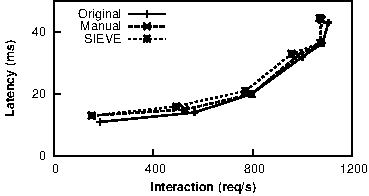
\includegraphics[width=0.85\textwidth]{./figures/sieve/eval/thlatpcw1dc.pdf}
\label{fig:thputLatencyTPCW}
%\end{minipage}
}
\par\bigskip
\subfloat[RUBiS bidding mix]{
\centering
%\begin{minipage}[b]{1.0\textwidth}
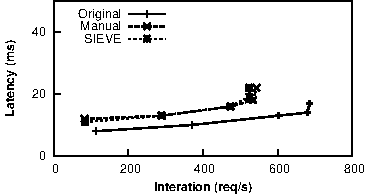
\includegraphics[width=0.85\textwidth]{./figures/sieve/eval/thlarubis1dc.pdf}
\label{fig:thputLatencyRUBiS}
%\end{minipage}
}
\caption{Throughput-latency graph without replication}
\label{fig:evalThroughputLatency}
\end{figure}

\paragraph{Correctness validation.} To verify that \tool\ labels operations correctly for
both case studies, we compared  the classification results
obtained by running \tool\ with TPC-W and RUBiS against
the results achieved manually in Chapter~\ref{chapter:redblue}.
Our finding in Table~\ref{tab:classfyresult} shows that
the percentage of shadow operations classified as red by \tool\ 
matches the results obtained through the manual classification.
In addition, a careful inspection of the logs shows that the expected pairs of functions and parameters 
were in fact labeled as red. This implies that \tool\ is able to achieve the same 
labeling as a manual process while saving a significant amount of effort from 
programmers and avoiding human mistakes.
% the log files generated by running
% \tool\ with TPC-W and RUBiS, and we found that \tool\ conducts the same 
% classification that was achieved manually in our previous work.
%  summarizes the classification results
% obtained both through manual classification and \tool.  
\begin{figure}[t!]
\centering
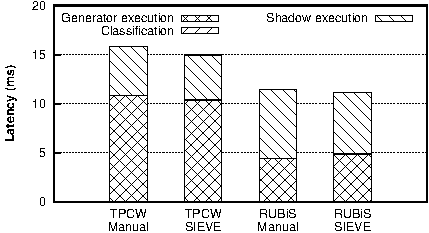
\includegraphics[width=0.85\textwidth]{./figures/sieve/eval/latencyBreakDownBar1.pdf}
\caption{Breakdown of latency.}
\label{fig:latencybreakdownbar}
\end{figure}

\paragraph{\tool\ runtime overhead.} Next we compared the performance
(throughput vs.\ latency) of the two applications across three
single-site deployments: 1) \tool, 2) Original---the original unreplicated
service without any overheads from creating and applying shadow
operations, and 3) Manual---the RedBlue scheme with all labeling
performed offline by the programmer. The expected sources of overhead
for \tool\ are: $i)$ the dynamic creation of shadow operations; and
$ii)$ the runtime classification of each shadow operation.  The
results in Figure~\ref{fig:evalThroughputLatency} show that the
performance achieved by \tool\ is similar to the one obtained with a
manual classification scheme, and therefore the overheads of runtime
classification are low. The comparison with the original scheme in a
single site shows some runtime overhead due to creating and applying
shadow operations (which is required for a replicated deployment so
that all operations commute).
%Also these results validate our expectations that the runtime overhead imposed by our
%mechanisms is negligible when compared with the unmodified use cases.

To better understand the sources of overhead imposed by \tool\ we
measured the latency contribution of each runtime step executed
by \tool\ and compared it with the latency contribution of these steps when relying on a manual
adaptation. In particular, we focused on the following tasks: generator execution (producing a shadow operation), classification (determining
shadow operation colors), and shadow execution (applying shadow operations). 

Figure~\ref{fig:latencybreakdownbar} shows the average contribution to request latency of
each of these steps (Only update requests are considered
since read-only queries do not generate side effects.) For the manual adaptation, there is no latency associated with classifying shadow operations, 
since the classification of all shadow operations is pre-defined. In contrast,
\tool\  performs a runtime classification, but the results show that the time consumed in this task is negligible. 
In particular,
% this takes is instantaneous (zero latency contribution) to
%verify weakest preconditions of read-only shadow operation (which are trivially blue). 
%for update shadow operations,
 \tool\ takes 0.064 $\pm$ 0.002 $ms$ and
0.072 $\pm$ 0.001 $ms$ for looking up the dictionary and evaluating
the condition for TPC-W and RUBiS, respectively. Regarding the
generator execution and shadow execution, both the manual adaptation and \tool\ present
the same latency overheads.


\if 0
Figure~\ref{fig:rubislatencybar} shows the average latency of every single interaction from
all deployments, namely original RUBiS, RUBiS with Gemini, and RUBiS
with \tool. From the results, we conclude that the overhead introduced by \tool\ is
very small. As shown in Figure~\ref{fig:rubislatencybar1}, \tool\ doesn't
add extra latency to each read-only interaction. The reason is that \tool\ will not
generate a shadow operation for any read-only transaction, and will not invoke
weakest precondition checking as well. As shown in Figure~\ref{fig:rubislatencybar2},
we add a small amount overhead to the updating interaction, but not much. Gemini manually
defines a set of shadow operation classes, and classify these classes as Red or Blue, statically.
Despite this, in order to create an instance to instantiate these classes, one using Gemini
has to inject codes inside applications to keep track of updates, and encode these updates into
the created instances. This part is as the same as what we are doing with \tool. The only difference
is that Gemini doesn't need runtime evaluation, but \tool\ does. However, the evaluation is 
lightweight.

\begin{figure*}[!ht]
\centering
\subfloat[Read-only interaction]{
%\begin{minipage}[b]{0.5\textwidth}
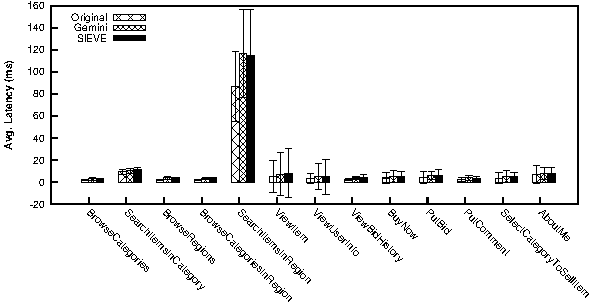
\includegraphics[height=0.33\textheight]{./figures/sieve/eval/rubisLatencyBarReadonly.pdf}
\label{fig:rubislatencybar1}
%\end{minipage}
}
\par\bigskip
%\hspace{0.4cm}
\subfloat[Update interaction]{
%\begin{minipage}[b]{0.5\textwidth}
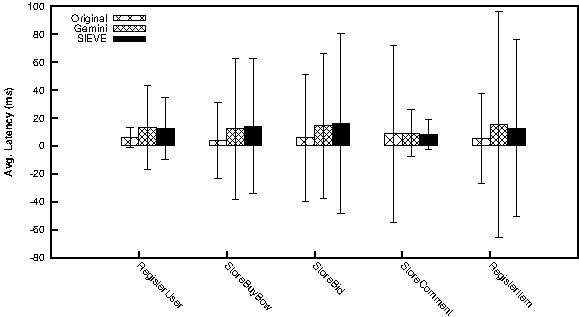
\includegraphics[height=0.33\textheight]{./figures/sieve/eval/rubisLatencyBarWrite.pdf}
\label{fig:rubislatencybar2}
%\end{minipage}
}
\caption{Average latency of different iterations. For other iterations
that don't have database access, the difference is negligible, so we
don't put into the figure.}
\label{fig:rubislatencybar}
\end{figure*}

Figure~\ref{fig:tpcwlatencybar} shows the comparison of the average
latency per interaction across three different deployments.

\begin{figure*}[!ht]
\centering
\subfloat[High latency]{
%\begin{minipage}[b]{0.5\textwidth}
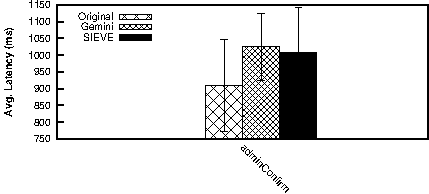
\includegraphics[height=0.33\textheight]{./figures/sieve/eval/tpcwLatencyBarhigh.pdf}
\label{fig:tpcwlatencybar1}
%\end{minipage}
}
%\hspace{0.4cm}
\par\bigskip
\subfloat[Low latency]{
%\begin{minipage}[b]{0.5\textwidth}
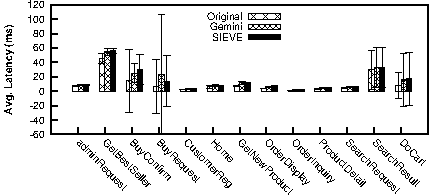
\includegraphics[height=0.33\textheight]{./figures/sieve/eval/tpcwLatencyBarlow.pdf}
\label{fig:tpcwlatencybar2}
%\end{minipage}
}
\caption{Average latency of different interactions. \cheng{The Gemini curve uses
the same data as SIEVE, since the data is not available now and my script
to build this chart requires three inputs.}}
\label{fig:tpcwlatencybar}
\end{figure*}
\fi

%\allen{Important graph/experiment that is missing is the comparison to
%  the hand-tuned implementations from OSDI.  Have we introduced
%  excessive overheads?}

\begin{figure}[t!]
\centering
\subfloat[TPC-W shopping mix]{
%\begin{minipage}[b]{0.5\textwidth}
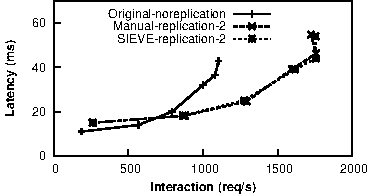
\includegraphics[width=0.86\textwidth]{./figures/sieve/eval/thlatpcwall.pdf}
\label{fig:thputLatencyTPCWRep}
%\end{minipage}
}
\par\bigskip
\subfloat[RUBiS bidding mix]{
%\begin{minipage}[b]{0.5\textwidth}
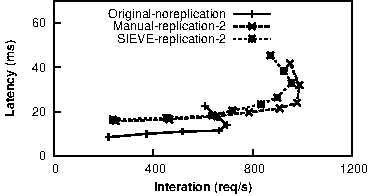
\includegraphics[width=0.86\textwidth]{./figures/sieve/eval/thlarubisall.pdf}
\label{fig:thputLatencyRUBiSRep}
%\end{minipage}
}
\caption{Throughput-latency graph with two replicas.}
\label{fig:evalThputLatency}
\end{figure}

\paragraph{Replication benefits.}
The results previously discussed in this section have shown that the
use of \tool\ imposes a small overhead when compared to a standalone
execution of the unmodified use cases, mostly due to runtime
classification. However, \tool\ was designed to allow replication to
bring performance gains through the use of weak consistency in
replicated deployments. To evaluate these benefits, we conducted an
experiment where we deployed the two applications (1) without
replication, (2) using manual classification in Gemini, and (3)
using \tool, with two replicas in the same site for the last two
options. (The use of single site replication instead of
geo-replication makes our results conservative, since the overheads of
runtime classification become diluted when factoring in cross-site
latency.) 

The results in Figure~\ref{fig:evalThputLatency} show that weakly consistent replication for a large
fraction of the operations brings performance gains. In particular, one
observes that the peak throughput with 2 replicated Gemini instances
running TPC-W is improved by 59.0\%, and the peak throughput for
RUBiS in this setting is improved by 37.4\%. %raw number (955-695)/695
The additional latency
introduced in this case is originated by the necessity of coordination
among replicas to totally order red shadow operations. The results
also confirm that the overhead of runtime classification when compared
to the manual, offline classification are low. Note that there is a
point where the throughput goes down while there is still an increase
in latency in Figure~\ref{fig:evalThputLatency}\subref{fig:thputLatencyRUBiSRep}. This happens
because the database becomes saturated at this point.
